\documentclass[12pt,article]{article}
\usepackage{fullpage}
\usepackage[top=2cm, bottom=4.5cm, left=2cm, right=2cm]{geometry}
\usepackage{amsmath,amsthm,amsfonts,amssymb,amscd}
\usepackage{lastpage}
\usepackage{enumerate}
\usepackage{fancyhdr}
\usepackage{mathrsfs}
\usepackage{xcolor}
\usepackage{graphicx}
\usepackage{listings}
\usepackage{hyperref}
\usepackage{mdframed}
\usepackage{changepage}   % for the adjustwidth environment
\usepackage{forest} 
\usepackage{tikz}   % For graph

\usepackage{float}  % To inforce inserting images at the right place

\usepackage{algorithm}
\usepackage{algpseudocode}

% For recursive formulation, adapted from https://tex.stackexchange.com/questions/580333/typing-sequences-recursively-in-overleaf
\usepackage{mathtools}
\makeatletter
\newcases{centercases}{\quad}
  {\hfil$\m@th\displaystyle{##}$\hfil}
  {$\m@th\displaystyle{##}$\hfil}{\lbrace}{.}
\makeatother

\newcommand{\Tau}{\mathrm{T}}


% For matrix
\def\horzbar{\text{magic}}

\hypersetup{%
  colorlinks=true,
  linkcolor=blue,
  linkbordercolor={0 0 1}
}

\setlength{\parindent}{0.0in}
\setlength{\parskip}{0.05in}

\newcommand\projnumber{1}
\newcommand\course{CS534}
\newcommand\OSUID{934370552}
\newcommand\Email{buivy@oregonstate.edu}
\newcommand\Name{Vy Bui}
\newcommand\tab[1][1cm]{\hspace*{#1}}

\pagestyle{fancyplain}
\headheight 35pt
\lhead{Homework \projnumber}
\rhead{Jan. 25, 2023}
\lfoot{}
\cfoot{}
\rfoot{\small\thepage}
\headsep 1.5em

\newenvironment{task}[2][Task]
    { \begin{mdframed}[backgroundcolor=gray!20] \textbf{#1 #2} \\}
    {  \end{mdframed}}
   

% Make Rightarrow with superscript
% \makeatletter
% \newcommand{\xRightarrow}[2][]{\ext@arrow 0359\Rightarrowfill@{#1}{#2}}
% \makeatother

\begin{document}

\begin{titlepage}
    \begin{center}
        \vspace*{4cm}

        \textbf{\Large AI539 - Natural Language Processing with Deep Learning}

        \vspace{0.5cm}
 
        \textbf{ Homework 1 Report}

        \textbf{ Word Vectors: Distributed Representations of Words}
 
        \vspace{1cm}

        Author: Vy Bui

        OSUID: 934370552

        \vspace{1cm}

        Instructor: Professor Stefan Lee
        \vfill
             
        \vspace{0.8cm}
      
             
        The School of Electrical Engineering and Computer Science\\
        Oregon State University\\
             
    \end{center}
\end{titlepage}

%==============================================================================%
\begin{task}{1.1} 
Implement the tokenize function in Vocabulary.py that processes a string into an array of strings corresponding to tokens. You are free to implement any tokenization schema that eliminates punctuation. If you want to try out lemmitization, the nltk package may be helpful. In your writeup for this question, include a description of what you implemented and include an example input-output pair.
\end{task}

remove punctuation and separate words by spaces.

There are still many other ways to try, like lemmatization or stemming, 

%==============================================================================%
\begin{task}{1.2} 
Implement the build\_vocab function in Vocabulary.py which constructs a finite vocabulary from a string containing all the text from the training corpus. This includes implementing some heuristic for thresholding the number of words and building the word2indx and idx2word indexes.
\end{task}

%==============================================================================%
\begin{task}{1.3} 
Implement the make\_vocab\_charts function in Vocabulary.py to produce Token Frequency Distribution and Cumulative Fraction Covered charts like those above for your tokenizer and vocabulary cutoff heuristic. We recommend matplotlib for this. Afterwards, running build\_freq\_vectors.py will generate these plots. In your write-up for this question, include these plots and briefly describe the cutoff heuristic you implemented and explain your rational for setting it.
\end{task}

%==============================================================================%
\newpage
\begin{task}{2.1}
What are the minimum and maximum values of PMI (Eq. 1)? If two tokens have a positive PMI, what does that imply about their relationship? If they have a PMI of zero? What about if the PMI is negative? Based on your answers, what is an intuition for the use of PPMI?
\end{task}

PMI values can go from negative infinity to positive infinity. If two tokens have a positive PMI, they co-occur more often than we expect by chance. Intuitively speaking, they tend to appear together in some predefined context. On the other hand, a negative PMI implies that the two tokens co-occur less often than expected by chance. A zero PMI implies that the probability that two tokens co-occur is just about the same as they occur together by chance. PPMI is favored because negative PMI is only reliable for immense corpora. Imagine two tokens each of which has probability of one millionth. To determine if two tokens co-occur less often than expected, the probability of the two appearing with one another has to have a magnitude of one thousand billionth, which requires a huge corpus \cite{JurafskyMartin08}.

%==============================================================================%
\begin{task}{2.2}
Implement the compute\_cooccurrence\_matrix function in build\_freq\_vectors.py which takes a list of article overviews and a vocabulary and produces a co-occurrence matrix C. It is up to the student to define what a context is. Note that looping in Python is quite slow such that unoptimized versions of this function can take quite a long time. Feel free to save the result while you are developing to reduce time in future runs (see numpy.save/numpy.load). In your writeup for this task, describe how you defined your context.
\end{task}

1. Context? \newline
2. 

%==============================================================================%
\begin{task}{2.3} 
Implement the compute\_ppmi\_matrix function in build\_freq\_vectors.py which calls 

compute\_cooccurrence\_matrix and then computes a PPMI matrix given a list of article overviews and a vocabulary. Hint: Add a small constant to C to avoid problems with log(0).
\end{task}

%==============================================================================%
\newpage
\begin{task}{2.4} 
It has all led up to this! Run build\_freq\_vectors.py and examine the visualized word vectors. You should have semantically meaningful clusters in your plot. Zoom in and identify three such clusters. In your write-up, include an image of each cluster and what category you think it is representing. Also include the plot as a whole.
\end{task}

PPMI seems to effectively draw the association between words. Figure \ref{fig:q2-country-cluster} shows a cluster of countries and georaphical locations such "US", "India", "Britain", and "China". Figure \ref{fig:q2-american-football} shows a cluster of words that are highly related to American football. More interestingly, figure \ref{fig:q2-middle-east} shows that the Middle East countries and cities often co-occur with war-related words such as "killing", "bomb", "hostage", and "violence". This seems to be the public image of the Middle East represented by the media.

\begin{figure}[H]
    \centering
    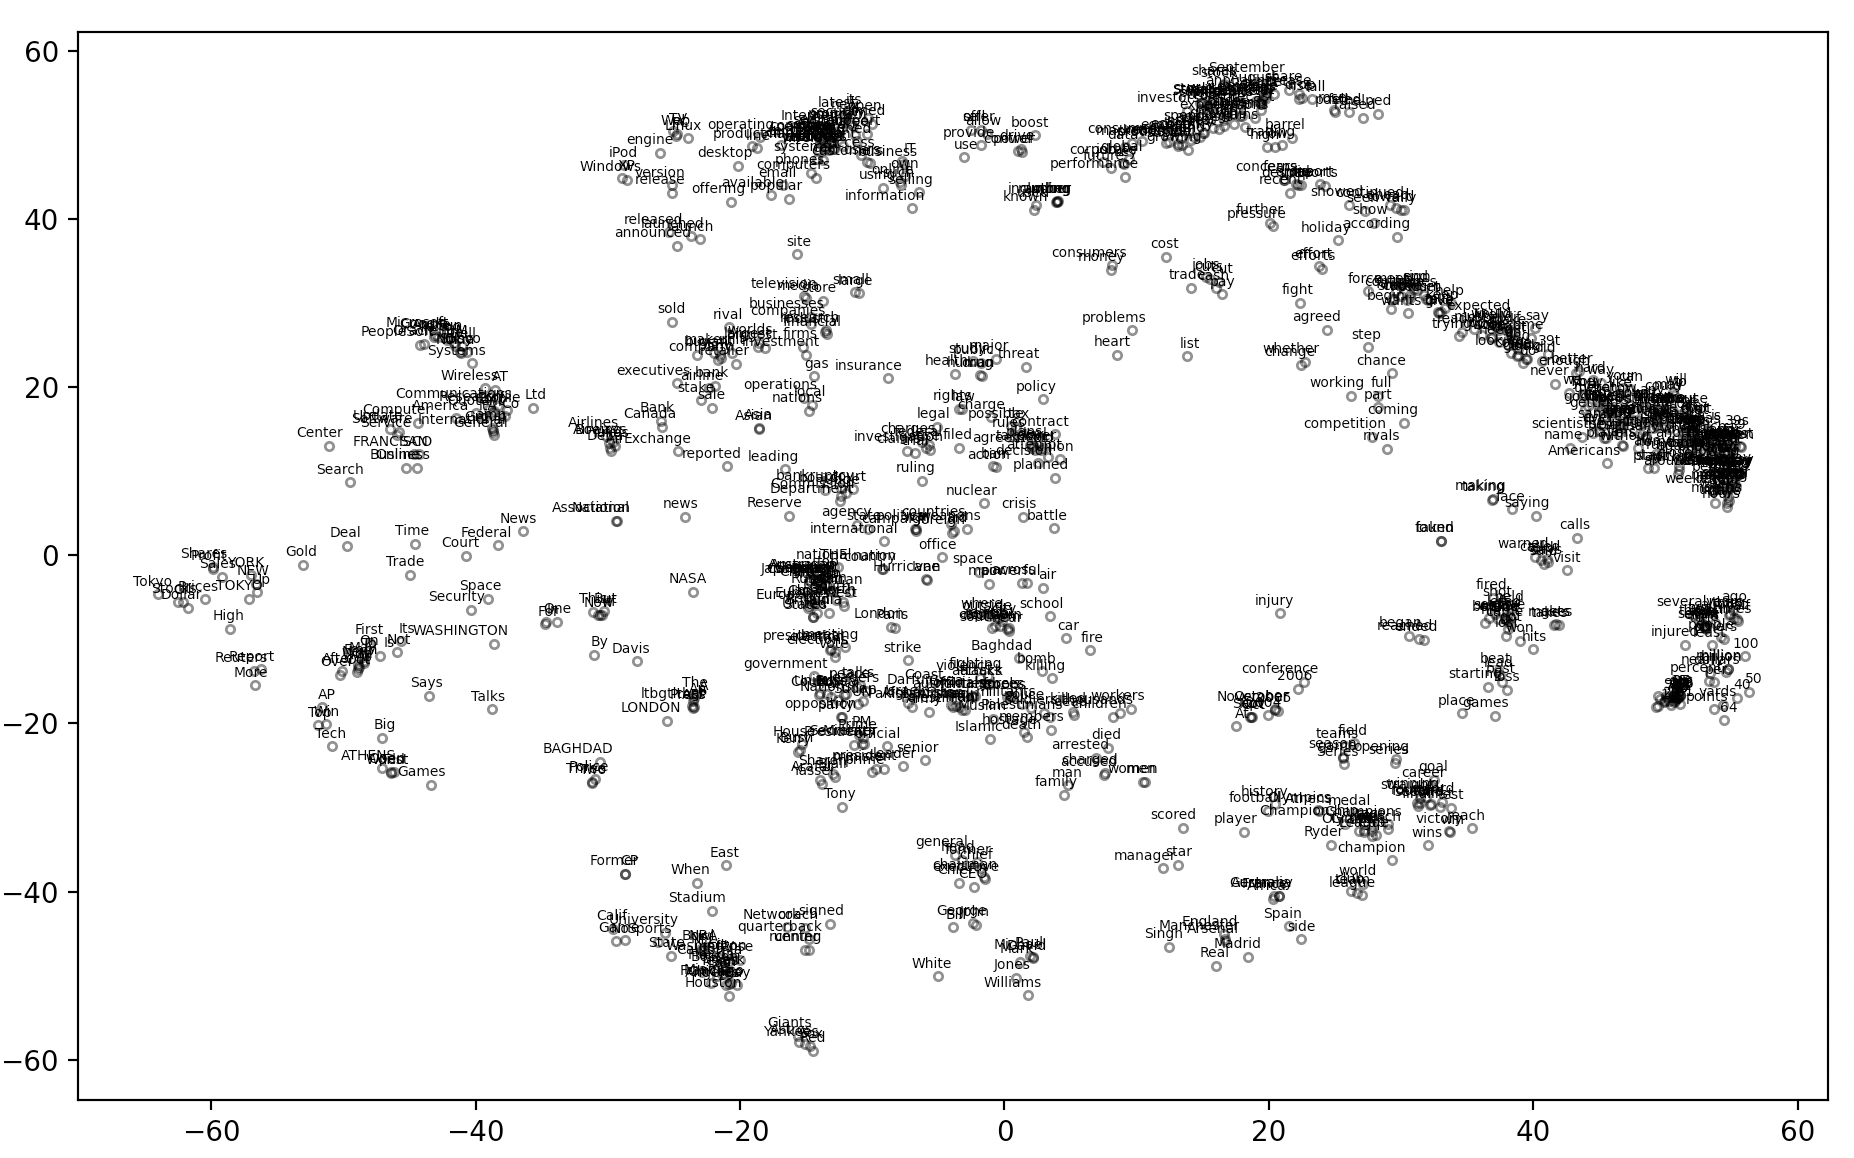
\includegraphics[scale=0.5]{whole_plot.png} \par
    \caption{Whole plot}
    \label{fig:q2-overview}
\end{figure}


\begin{figure}[H]
    \centering
    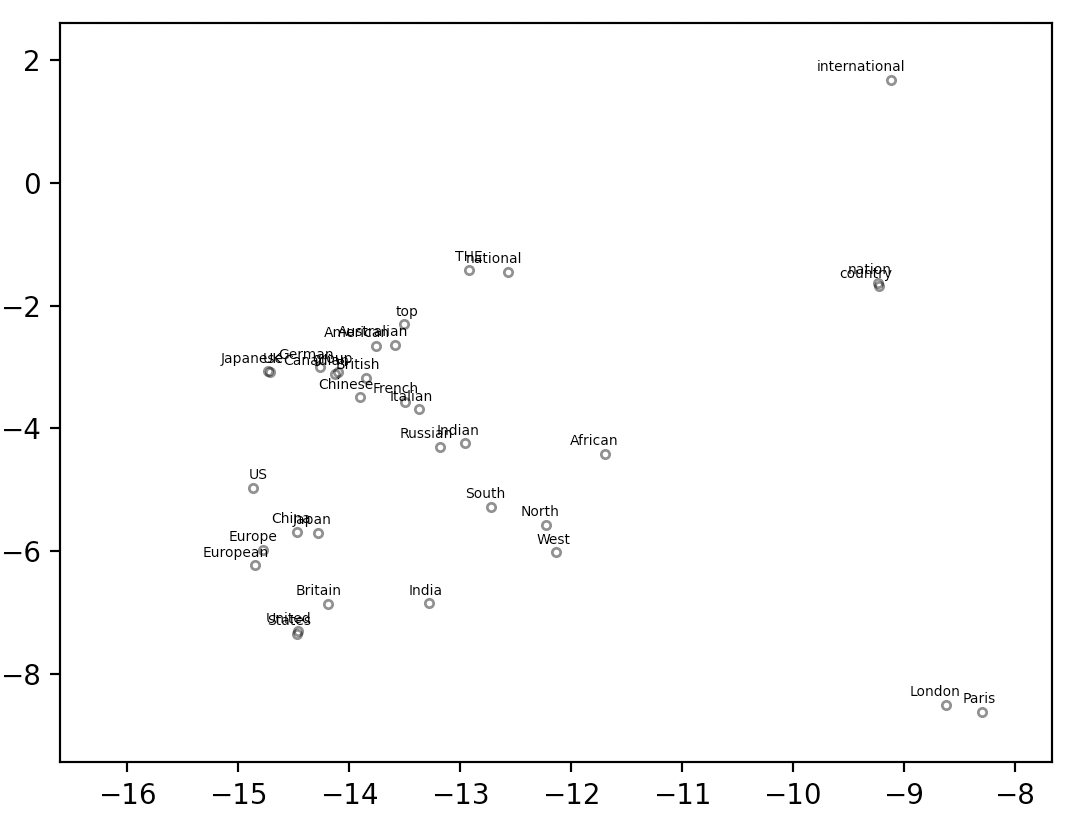
\includegraphics[scale=0.6]{country.png} \par
    \caption{Country cluster}
    \label{fig:q2-country-cluster}
\end{figure}


\begin{figure}[H]
    \centering
    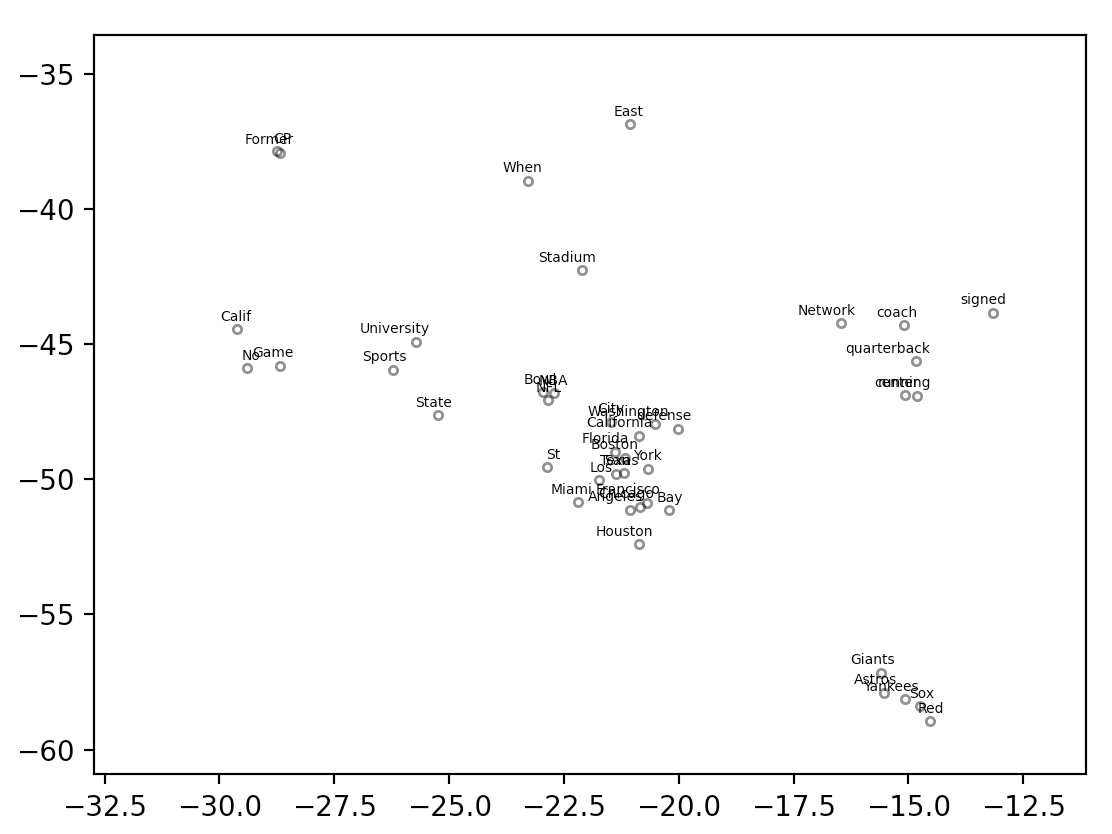
\includegraphics[scale=0.6]{american_football.png} \par
    \caption{American football cluster}
    \label{fig:q2-american-football}
\end{figure}


\begin{figure}[H]
    \centering
    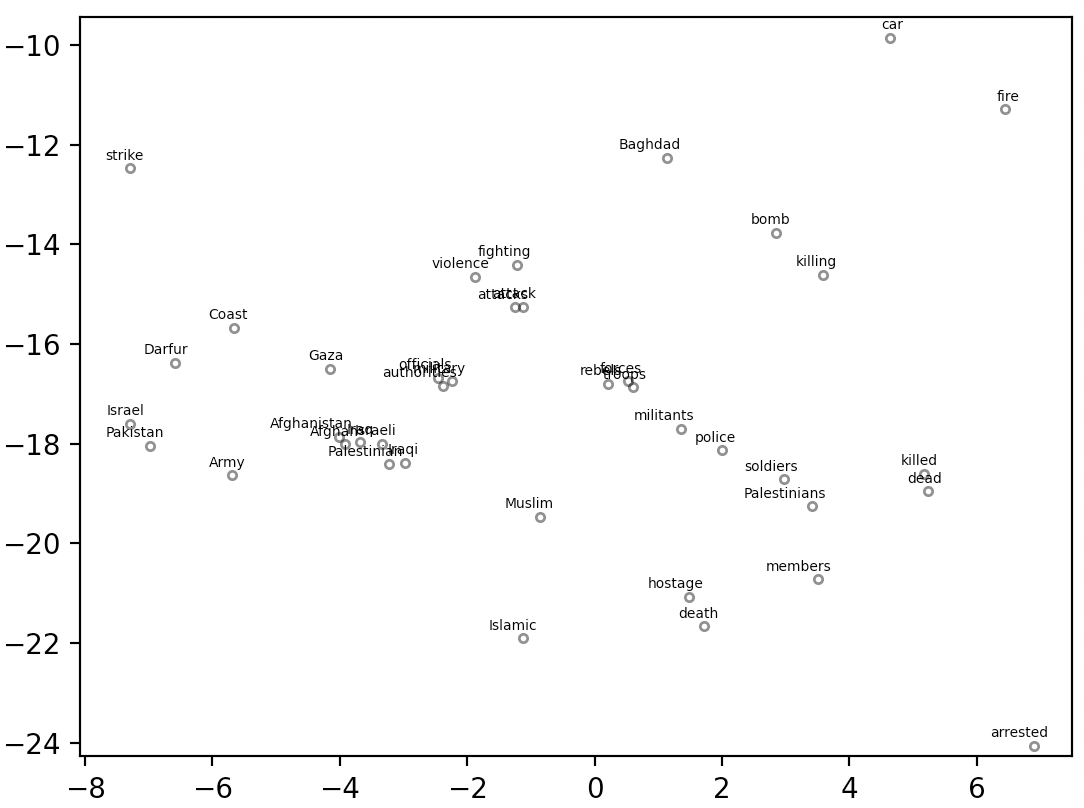
\includegraphics[scale=0.6]{middleeast_war.png} \par
    \caption{Middle East war cluster}
    \label{fig:q2-middle-east}
\end{figure}

%==============================================================================%
\newpage
\begin{task}{3.1}
Derive the gradient of the objective $J_B$ with respect to the model parameters $w_i, \widetilde{w}_j, b_i, \widetilde{b}_j$. That is, write the expression for $\triangledown_{w_i}J, \triangledown_{\widetilde{w}_j}J, \triangledown_{b_i}J, \triangledown_{\widetilde{b}_j}J$. Note that parameters corresponding to words not in B will have zero gradient.
\end{task}

%==============================================================================%
\begin{task}{3.2} 
Implement the gradient computation for a batch in the corresponding Task 3.2 section of build\_glove\_vectors.py.
\end{task}

%==============================================================================%
\begin{task}{3.3} 
Run build\_glove\_vectors.py to learn GloVe vectors and visualize them with TSNE! In your write-up, describe how the loss behaved during training (how stably it decreased, what it converged to, etc). Also include the TSNE plot. If everything has been done correctly, you should observe similar clustering behavior as in Task 2.3.
\end{task}

%==============================================================================%
\newpage
\begin{task}{4.1} 
Use the most\_similar function to find three additional analogies that work. In your response, provide the analogies in the compact a:b::c:? form, the model's list of outputs, and why you consider this output to satisfy the analogy.
\end{task}

%==============================================================================%
\begin{task}{4.2} 
Use the most\_similar function to find three analogies that did not work. In your response to this question, provide the analogies in the compact a:b::c:? form, the model's list of outputs, and why you consider this output to not satisfy the analogy.
\end{task}

%==============================================================================%
\begin{task}{4.3} 
Use the most\_similar function to find two additional cases of bias based on gender, politics, religion, ethnicity, or nationality. In your response, provide the analogies in the compact a:b::c:? form, the model's list of outputs for both a:b::c:? and c:b::a:?, and why you consider this output to be biased based on the model's two responses.
\end{task}

%==============================================================================%
\begin{task}{4.4} 
Why might these biases exist in word2vec and what are some potential consequences that might result if word2vec were used in a live system?
\end{task}

\bibliographystyle{alpha}
\bibliography{mybib}
\end{document}
